\documentclass[a4paper,11pt]{jsarticle}


% 数式
\usepackage{amsmath,amsfonts}
\usepackage{bm}
\usepackage{physics}
% 画像
\usepackage[dvipdfmx]{graphicx}
% ローマ数字
\usepackage{otf}
% 単位
\usepackage{siunitx}
% 表
\usepackage{multirow}
% 化学反応
\usepackage[version=4]{mhchem}
\usepackage{url}

\begin{document}

\title{素粒子物理学 後半レポート}
\author{05-211525 齋藤駿一}
\date{\today}
\maketitle

\section*{1}

\begin{align}
  \alpha(Q) &= \frac{\alpha(\mu)}{1-\frac{\alpha(\mu)}{3\pi}\ln{\frac{Q^2}{\mu^2}}} \\
  \alpha_S(Q) &= \frac{\alpha_S(\mu)}{1-b_0\alpha_S(\mu)\ln{\frac{Q^2}{\mu^2}}} 
\end{align}
が成り立つ.
ただし,
\begin{equation}
  b_0 = - \frac{11N_c - 2N_f}{12\pi}
\end{equation}
である.
まず,$\mu=m_e=\SI{511}{\keV}$として$\alpha(m_e)=1/137$を用いると,
\begin{equation}
  \alpha(Q) = \frac{1/137}{1-\frac{1/137}{3\pi}\ln{\frac{Q^2}{m_e^2}}}
\end{equation}
がいえる.

いま,$N_c=3,\,N_f=5$の場合を考えて,$b_0\approx -0.6101$
とする.
$\mu=\SI{91.2}{\GeV}$として$\alpha_S(\SI{91.2}{\GeV})=0.119$を用いると,
\begin{equation}
  \alpha_S(Q) = \frac{0.119}{1+0.6101\times0.119\ln{\frac{Q^2}{\SI{91.2}{\GeV}^2}}}
\end{equation}
がいえる.

以上をもとに表を埋めると,次のようになる.

\begin{table}[htbp]
  \centering
  \caption{QED couplingとQCD couplingの表.}
  \label{tab:couplconst}
  \begin{tabular}{c|c|c|c|c|c}
    \hline
    Q & \SI{10}{\GeV} & \SI{100}{\GeV} & \SI{1}{\TeV} & \SI{1.75}{\TeV} & \SI{1.15e19}{\eV} \\
    \hline\hline
    QED $\alpha$ & $7.58\times 10^{-3}$ & $7.61\times 10^{-3}$ & $7.63\times 10^{-3}$ & - & $1.05\times 1/137$\\
    \hline
    QCD $\alpha_S$ & $1.78\times10^{-2}$ & $1.69\times 10^{-2}$ & $1.62\times10^{-2}$ & $0.119\times 0.7$ & - \\
    \hline
  \end{tabular}
\end{table}

\section*{2}

\subsection*{Q1}
%Muon Lifetime 読んで適当に埋める.
崩壊反応$\mu \to e^- +\bar{\nu}_e+ \nu_{\mu}$のFeynman diagramに対しFeynman ruleを適用すると,
\begin{equation}
  \mathcal{M} = i\frac{ig_{\mu\nu}}{M_W^2}\bar{u}(k_2,s_2)\left(-i\frac{g}{\sqrt{2}}\gamma^\mu\frac{1}{2}(1-\gamma^5)\right)u(k_1,s_1)\bar{u}(k_4,s_4)\left(-i\frac{g}{\sqrt{2}}\gamma^\nu\frac{1}{2}(1-\gamma^5)\right)u(k_3,s_3)
\end{equation}
と書ける.
ただし,$\mu,\nu_{\mu},\nu_{e},e^-$をそれぞれ粒子1,2,3,4とラベルした.
これをFermi定数
\begin{equation}
  G_F = \frac{\sqrt{2}g^2}{8M_W^2}
\end{equation}
を用いて整理すると,
\begin{equation}
  \mathcal{M} = \frac{G_F}{\sqrt{2}}\bar{u}(k_2,s_2)\gamma^\mu (1-\gamma^5)u(k_1,s_1)\bar{u}(k_4,s_4)\gamma^\nu (1-\gamma^5)u(k_3,s_3)
\end{equation}
となる.
これをもとにトレース計算すると,
\begin{equation}
  \left|\mathcal{M}\right|^2 = 64G_F^2(k_1\cdot k_3)(k_2 \cdots k_4)
\end{equation}
が分かる.
これを
\begin{equation}
  d\Gamma = \frac{1}{2m_{\mu}}\left|\mathcal{M}\right|^2 \frac{d^3k_2}{(2\pi)^3 2E_2}\frac{d^3k_3}{(2\pi)^3 2E_3}\frac{d^3k_4}{(2\pi)^3 2E_4} (2\pi)^4\delta^4(k_1-k_2-k_3-k_4)
\end{equation}
に代入し,さらに計算すると,
\begin{equation}
  \frac{d\Gamma}{dE} = \frac{m_{\mu}^2G_F^2}{4\pi^3}E^2\left(1-\frac{4E}{3m_{\mu}}\right)
\end{equation}
が分かる.
これを$E=0$から$E=m_{\mu}/2$(右辺の微分がゼロになるエネルギー)まで積分すると,
\begin{equation}
  \Gamma = \frac{G_F^2 m_{\mu}^5}{192\pi^3}
\end{equation}
と求まる.
したがって,$\mu$粒子の寿命は
\begin{equation}
  \tau = \frac{1}{\Gamma} = \frac{192\pi^3}{G_F^2 m_{\mu}^5}
\end{equation}
と求まる.

\begin{thebibliography}{99}
  \bibitem{muon} A.George. (2012). Muon \& Tau Lifetime.\\
  \url{http://hep.ucsb.edu/people/cag/Muon_Lifetime.pdf}
\end{thebibliography}

\subsection*{Q2}

\begin{equation}
  \tau_{\mu} = \frac{192\pi^3}{G_F^2m_{\mu}^5}= \frac{192\pi^3\hbar}{\left(\frac{G_F}{(\hbar c)^3}\right)^2(m_{\mu}c^2)^5}
\end{equation}
に
\begin{equation}
  \frac{G_F}{(\hbar c)^3} = \SI{1.1663789e-5}{\GeV^{-2}}, \, m_{\mu}c^2 = \SI{105.65837}{\MeV},\, \hbar = \SI{6.582119569e-22}{\MeV \s}
\end{equation}
を代入すると,
\begin{equation}
  \tau_{\mu} \approx \SI{2.187347816e-6}{\s}
\end{equation}
と求まる.

\subsection*{Q3}
PDGで検索すると,
\begin{equation}
  \tau_{\mu} = \SI[separate-uncertainty=true]{2.1969811+-0.0000022e-6}{\s}
\end{equation}
と分かった.
先ほどの計算結果はこれよりも有意に小さい.

\section*{3}
%Youtube check!
ニュートリノのヘリシティを測定するには,次のGoldhaber experimentを行えば良い.
まず,スピン$l=0$の原子核$X$で,K殻の電子捕獲によりスピン$l=1$の原子核$Y^*$に励起するものを用意する.
すなわち,
\begin{equation}
  X + e^- \to Y^* + \nu_{e}
\end{equation}
が起こると考える.
電子捕獲のとき系全体は静止しているので,運動量保存により終状態の全運動量は0である.

さらに,励起された原子核が光子を放出してスピン$l=0$の基底状態$Y$へ遷移すると考える.
すなわち,
\begin{equation}
  Y^* \to Y + \gamma
\end{equation}
が起こると考える.
前述したように終状態の全運動量は0であり,原子核は静止していると考えれば,ここで放出される光子の運動量$\bm{p}_{\gamma}$と電子ニュートリノの運動量$\bm{p}_{\nu_e}$は
\begin{equation}
  \bm{p}_{\gamma} = -\bm{p}_{\nu_e}
\end{equation}
を満たす.

ここで,系全体のスピンのz成分が反応全体
\begin{equation}
  X + e^- \to Y + \gamma + \nu_{e}
\end{equation}
を通して保存することを考えると,各粒子のスピンのz成分の組として
\begin{equation}
  0 + \frac{1}{2} \to 0 + 1 - \frac{1}{2} 
\end{equation}
または
\begin{equation}
  0 - \frac{1}{2} \to 0 - 1 + \frac{1}{2} 
\end{equation}
の2通りだけ考えられる.
したがって,光子のスピン$\bm{s}_{\gamma}$と電子ニュートリノのスピン$\bm{s}_{\nu_e}$は必ず
\begin{equation}
  \bm{s}_{\gamma} = -\bm{s}_{\nu_e}
\end{equation}
を満たす.

以上より,光子のヘリシティ$h_{\gamma}$は電子ニュートリノのヘリシティ$h_{\nu_e}$と等しいことが分かる:
\begin{equation}
  h_{\gamma} = \frac{\bm{p}_e\cdot \bm{s}_e}{\left|\bm{p}_e\right|\cdot\left|\bm{s}_e\right|} = \frac{(-\bm{p}_{\nu_e})\cdot (-\bm{s}_{\nu_e})}{\left|-\bm{p}_{\nu_e}\right|\cdot\left|-\bm{s}_{\nu_e}\right|} =  h_{\nu_e}.
\end{equation}
つまり,光子のヘリシティを測定することで,間接的に電子ニュートリノのヘリシティを測定できる.

実際のGoldhaber experimentでは,\ce{^{152} Eu}が電子捕獲により\ce{^{152} Sm}となる反応が用いられた.
その結果,ニュートリノヘリシティは$-1$と求まり,ニュートリノは必ず左巻きになることが分かった.

\begin{thebibliography}{99}
  \bibitem{youtube} Manmohan Singh. Measurement of Helicity of Neutrino (Goldhaber Experiment). \\
  \url{https://www.youtube.com/watch?v=6ZaG5LFKmaI} 
\end{thebibliography}

\section*{4}

Zボソンの崩壊$\ce{Z -> f}\bar{\mathrm{f}}$の部分幅$\Gamma(\ce{Z -> f}\bar{\mathrm{f}})$は,
\begin{equation}
  \Gamma(\ce{Z -> f}\bar{\mathrm{f}}) = \frac{(G_F/(\hbar c)^3) m_{\mathrm{Z}}^3c^6}{3\pi\sqrt{2}} (c_{\mathrm{L}}^2+c_{\mathrm{R}}^2) \approx \SI{663}{\MeV} \cdot (c_{\mathrm{L}}^2+c_{\mathrm{R}}^2)
\end{equation}
を満たす.
ただし,
\begin{equation}
  c_{\mathrm{L,R}} = T_3 - \sin^2{\theta_W}Q \approx T_3 - 0.23\times Q
\end{equation}
である($c_{\mathrm{R}}$については$T_3 = 0$).
これをもとに部分幅を計算すると,表\ref{tab:c}のようになる.
ここで,クォークは3つの色の組み合わせで生成されることを考慮した.

\begin{table}[htbp]
  \centering
  \caption{各fについての$T_3 - \sin^2{\theta_W}Q$の値と部分幅.}
  \label{tab:c}
  \begin{tabular}{c|cc|cccc}
    \hline
    & $Q$ & $T_3$(Lのとき) & $c_{\mathrm{L}}$ & $c_{\mathrm{R}}$ & $c_{\mathrm{L}}^2+c_{\mathrm{R}}^2$ & $\Gamma/\si{\MeV}$ \\
    \hline\hline
    $\nu_e, \nu_{\mu}, \nu_{\tau}$ & 0 & 1/2 & 1/2 & 0 & 0.25 & 166 \\
    $\ce{e^-, \mu^-, \tau^-}$ & $-1$ & $-1/2$ & $-0.27$ & 0.23 & 0.13 & 83.4 \\
    $\ce{u, c}$ & 2/3 & 1/2 & 0.35 & $-0.15$ & 0.15 & 3$\times$94.8 \\
    $\ce{d, s, b}$ & $-1/3$ & $-1/2$ & $-0.42$ & 0.08 & 0.18 & 3$\times$123 \\
    \hline
  \end{tabular}
\end{table}
以上より,全幅は
\begin{equation}
  \Gamma_{\mathrm{tot}} = 3\times \SI{166}{\MeV} + 3\times \SI{83.4}{\MeV} + 2\times 3\times \SI{94.8}{\MeV} + 3\times 3\times \SI{123}{\MeV}  = \SI{2424}{\MeV}
\end{equation}
と計算できる.
これより,分岐比は
\begin{align}
  \mathrm{BR}(\ce{Z -> e^-e^+}) &= \frac{\Gamma(\ce{Z -> e^-e^+})}{\Gamma_{\mathrm{tot}}} \approx 0.0344\\
  \mathrm{BR}(\ce{Z -> invisible})/3 &= \frac{\Gamma(\ce{Z -> \nu_e}\bar{\nu_e})}{\Gamma_{\mathrm{tot}}} \approx 0.068\\
  \mathrm{BR}(\ce{Z -> }d\bar{d}+s\bar{s}+b\bar{b})/3 &= \frac{3\times\Gamma(\ce{Z -> }d\bar{d})}{\Gamma_{\mathrm{tot}}} \approx 0.152 \\
  \mathrm{BR}(\ce{Z -> }u\bar{u}+c\bar{c})/2 &= \frac{3\times\Gamma(\ce{Z -> }u\bar{u})}{\Gamma_{\mathrm{tot}}} \approx 0.117
\end{align}
と計算でき,これは実験結果とおおよそ合致する.

\begin{thebibliography}{99}
  \bibitem{text1} B.ポッフ,K.リーツ,C.ショルツ,F.サッチャ.柴田利明訳.素粒子・原子核物理入門.p.143
\end{thebibliography}

\section*{5}
観測されるHiggs粒子の個数$\tilde{N}$は,実際に生成される個数$N$を用いて,
\begin{equation}
  \tilde{N} = N\times \mathrm{Br}(H \ce{->} \mu^+\mu^-)\times 0.49
\end{equation}
と書ける.
ここで,integrated luminosity $L_{\mathrm{int}}$は,$N$と散乱断面積$\sigma$を用いて
\begin{equation}
  L_{\mathrm{int}} = \frac{N}{\sigma}
\end{equation}
と表される.
いま,すべての生成過程について散乱断面積を足し上げると,
\begin{equation}
  \sigma = \SI{43.9}{pb} + \SI{3.7}{pb} + \SI{1.4}{pb} + \SI{0.9}{pb} + \SI{0.5}{pb} = \SI{50.4}{pb}
\end{equation}
が得られるので,$L_{\mathrm{int}}=\SI{140}{fb^{-1}}$より
\begin{equation}
  N = L_{\mathrm{int}}\times\sigma \approx \SI{7.06e6}{}
\end{equation}
が分かる.

\subsection*{Q1}
Case Aでは,
\begin{equation}
  \mathrm{Br}(H \ce{->} \mu^+\mu^-) = 0.00022
\end{equation}
なので,観測されるHiggs粒子の個数は
\begin{equation}
  N \approx 761
\end{equation}
と求まる.

\subsection*{Q2}
Case Bでは,
\begin{equation}
  \mathrm{Br}(H \ce{->} \mu^+\mu^-) = 0.063
\end{equation}
なので,観測されるHiggs粒子の個数は
\begin{equation}
  N \approx \SI{2.18e5}{}
\end{equation}
と求まる.

\subsection*{Q3}
% 1807.06325.pdf check!
Search for the Higgs boson decaying to two muons in proton-proton collisions at $ \sqrt{s} = \SI{13}{\TeV}$

\subsection*{Q4}
Case Aが支持される.

\subsection*{Q5}
%飛ばす

\section*{6}
\subsection*{Q1,Q2}
図\ref{fig:fd}に示した.

\begin{figure}[htbp]
  \centering
  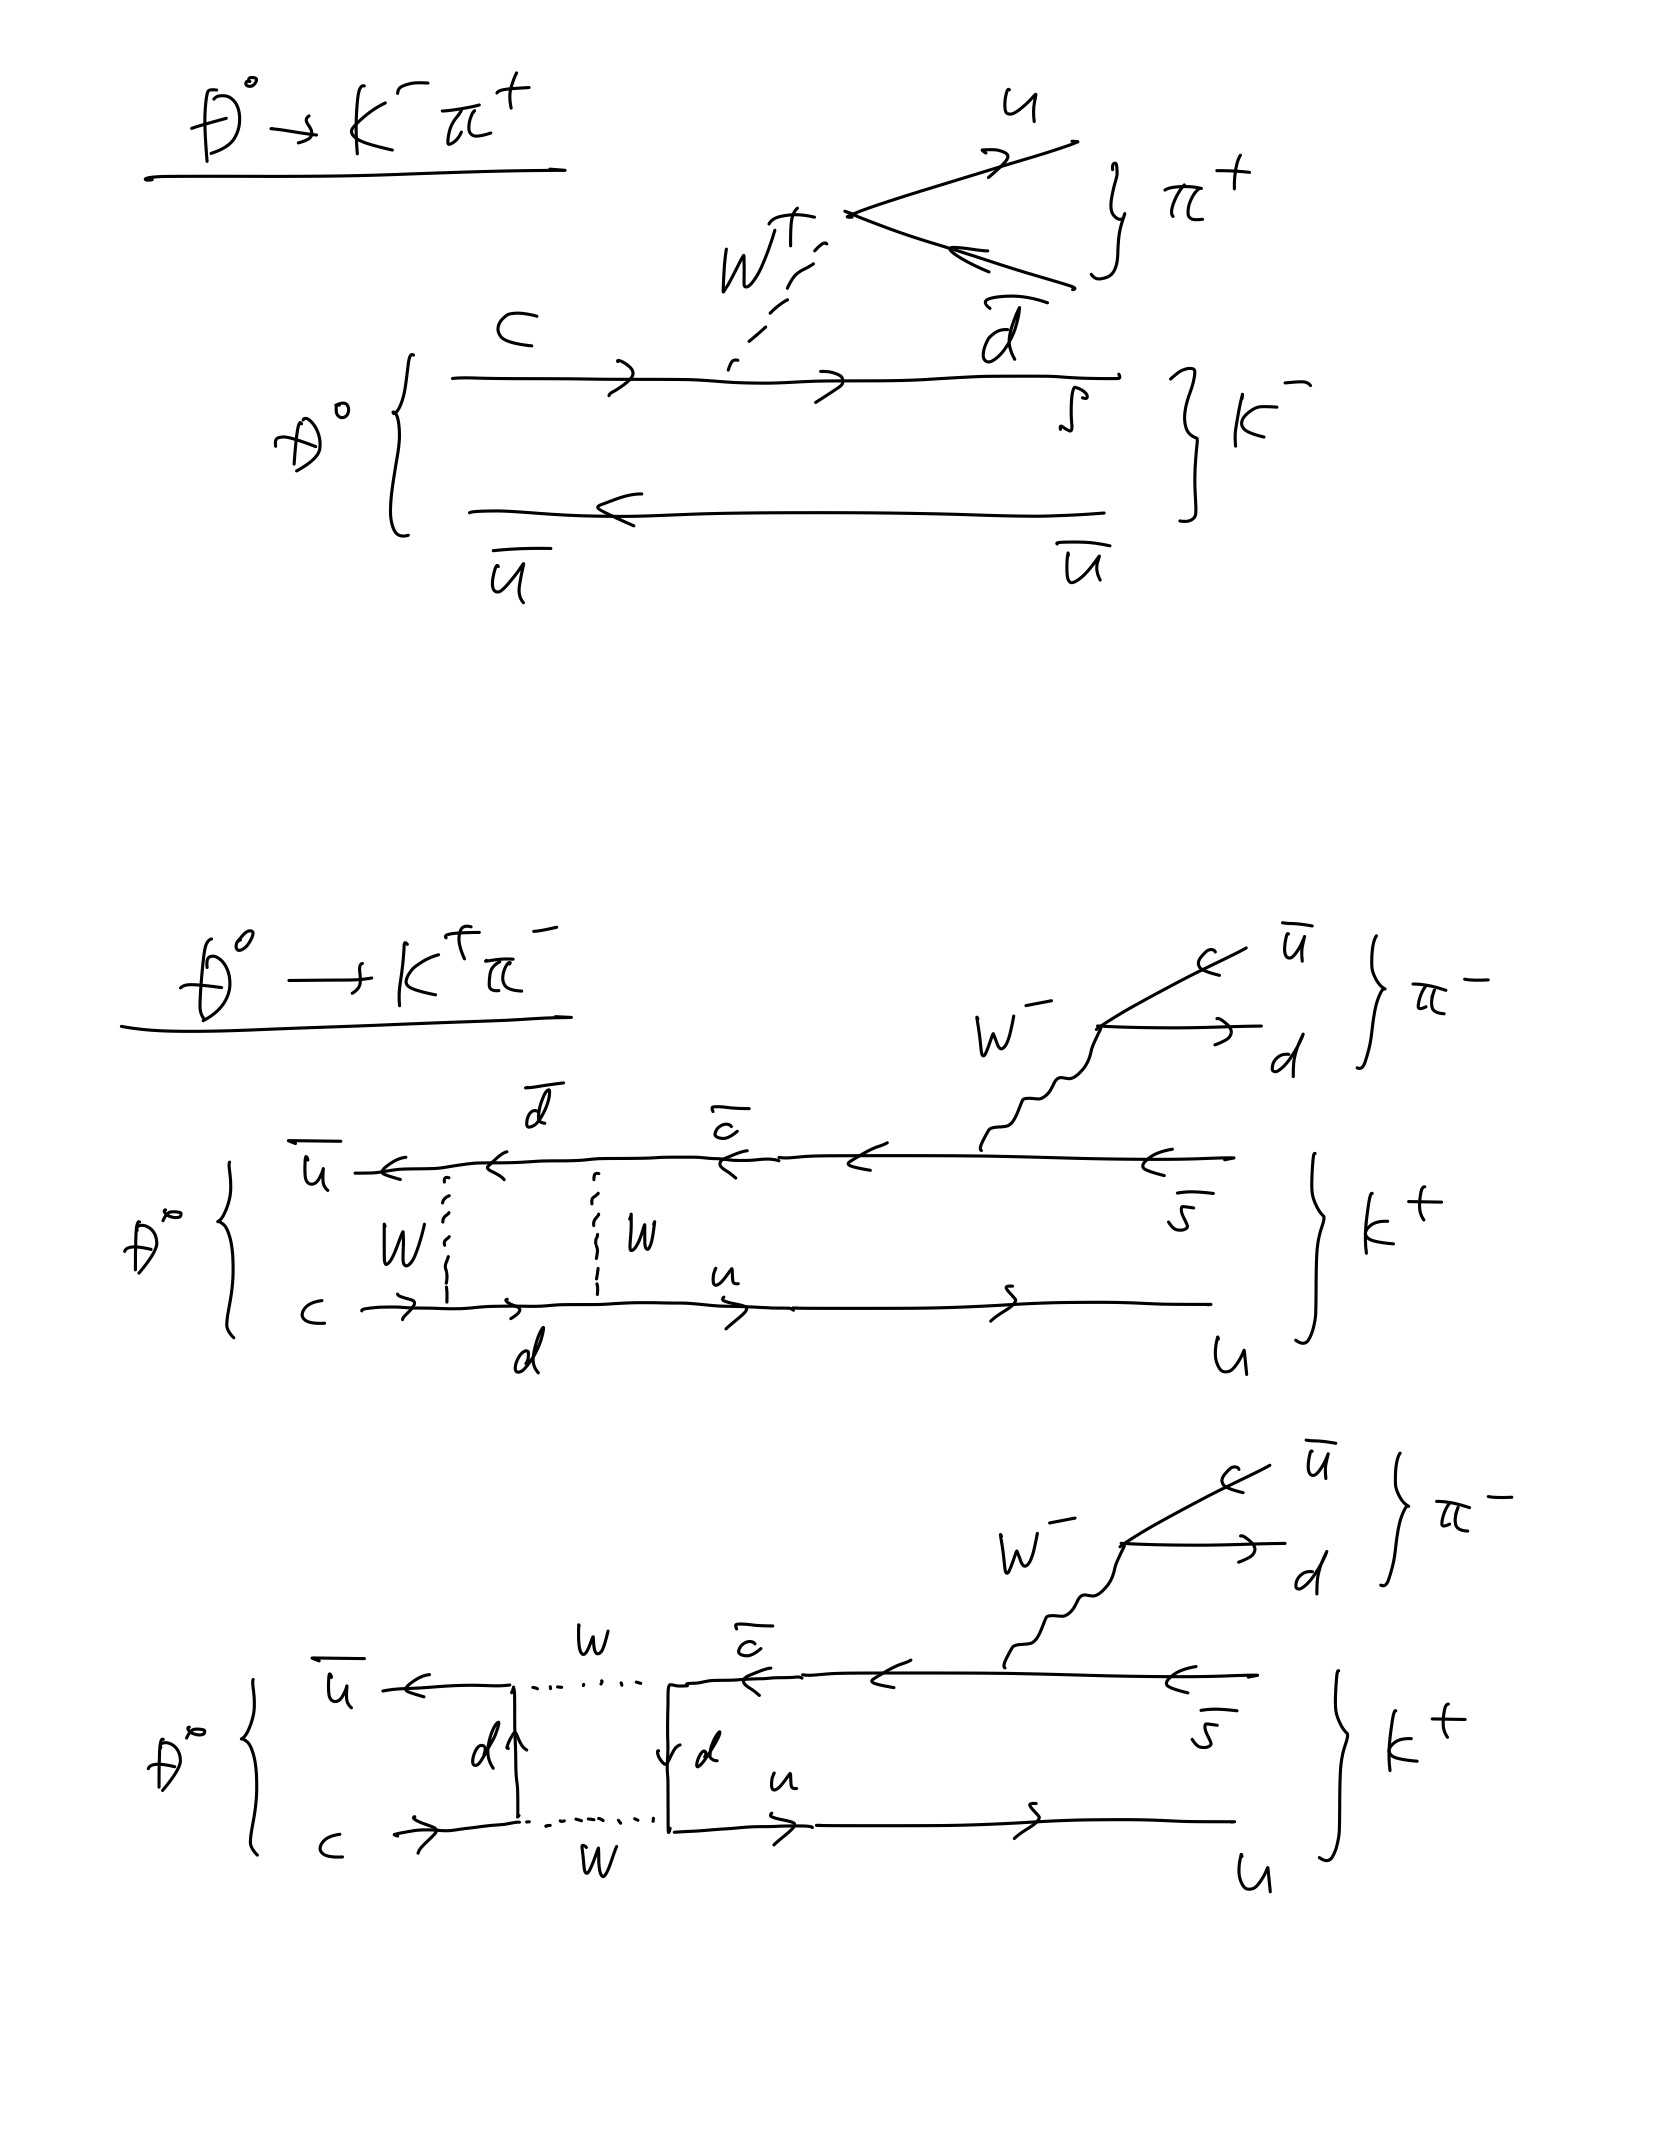
\includegraphics[width=10cm]{report_particle_physics_2022_tanaka-14.jpg}
  \caption{Q1の回答(上)とQ2の回答(下).}
  \label{fig:fd}
\end{figure}

\subsection*{Q3}
\ce{D^0\to K^+\pi^-}の反応では,図\ref{fig:fd}より,cクォークがdクォークに変わる必要がある.
これは,dクォークが実際にはsクォークと重ね合わさった状態として存在しているからであると考えられる.
重ね合わせの比率は,Cabbibo angle $\theta_C$を用いて
\begin{equation}
  \left(
  \begin{matrix}
    d'\\
    s'
  \end{matrix}
  \right)
  =
  \left(
  \begin{matrix}
    \cos{\theta_C} & \sin{\theta_C} \\
    -\sin{\theta_C} & \cos{\theta_C}
  \end{matrix}
  \right)
  \left(
  \begin{matrix}
    d \\
    s
  \end{matrix}
  \right)
\end{equation}
と書ける.
いま,$\sin{\theta_C}\approx 0.22, \cos{\theta_C}\approx 0.98$である.
したがって,\ce{c <-> d}の遷移確率は\ce{c <-> s}の遷移確率に比べて,
\begin{equation}
  \frac{\sin^2{\theta_C}}{\cos^2{\theta_C}} \approx \frac{1}{20}
\end{equation}
倍程度小さくなる.
\ce{D^0\to K^+\pi^-}の反応ではこれが2回起こるため,\ce{D^0\to K^-\pi^+}と比べて遷移確率は$1/400= 5\times 10^{-3}$倍程度になると考えられる.
これは実際の分岐比の割合$\SI{3.6e-3}{}$と概ね合致する.

\begin{thebibliography}{99}
  \bibitem{text2} B.ポッフ,K.リーツ,C.ショルツ,F.サッチャ.柴田利明訳.素粒子・原子核物理入門.p.129
\end{thebibliography}

\section*{7}
\ce{B^0}と\ce{\bar{B}^0}のmixingは因子$\cos{\Delta m_{\ce{B^0}}}$で表されるので,その周期は
\begin{equation}
  \frac{2\pi}{\Delta m_{\ce{B^0}}} = \frac{2\pi}{\SI{0.507}{ps}} = \SI{12.4}{ps}
\end{equation}
と分かる.
\ce{B^0_S}と\ce{\bar{B}^0_S}のmixingの周期も同様に,
\begin{equation}
  \frac{2\pi}{\Delta m_{\ce{B^0_S}}} = \frac{2\pi}{\SI{17.8}{ps}} = \SI{0.353}{ps}
\end{equation}
と分かる.
よって,粒子の速度を$\beta c$とすると,\ce{B^0}-\ce{\bar{\mathrm{B}}^0} mixingと\ce{B^0_S}-\ce{\bar{\mathrm{B}}^0_S} mixingのdecay lengthはそれぞれ
\begin{align}
  \beta c \times \SI{12.4}{ps} &\approx \SI{3.72}{mm}\times\beta  \\
  \beta c \times \SI{0.507}{ps} &\approx \SI{106}{\um}\times\beta  
\end{align}
と求まる.
これより,\ce{B^0_S}-\ce{\bar{\mathrm{B}}^0_S} mixingは,$\beta=1$としても$\sigma_{\Delta z} \approx \SI{100}{\um}$で判定できる限界の長さに近い.
実際は$\beta$はもっと小さいので,\ce{B^0_S}-\ce{\bar{\mathrm{B}}^0_S} mixingは観測できない.

\end{document}